%----------------------------------------
% Preamble to set up the document
%----------------------------------------
\documentclass{article}

% set up packages (you shouldn't need to touch this)
\usepackage{graphicx}  % required to insert images
\usepackage{hyperref}  % for hyperlinks
\usepackage[svgnames]{xcolor}  % to change hyperlink colors
\colorlet{linkcolour}{DarkBlue}
\hypersetup{colorlinks=true, linkcolor=linkcolour, citecolor=linkcolour, urlcolor=linkcolour,}

% Margins
\topmargin=-0.45in
\evensidemargin=0in
\oddsidemargin=0in
\textwidth=6.5in
\textheight=9.0in
\headsep=0.25in

% use a sans serif font
\renewcommand{\familydefault}{\sfdefault}

%----------------------------------------
% Step 1: Edit the lecture title
%----------------------------------------
\title{
Lecture 2: Introduction to Counting \\  % Lecture title
Modeling Social Data, Spring 2017 \\   % Course title
Columbia University                    % School
}

%----------------------------------------
% Step 2: Edit your name and the date
%----------------------------------------
\author{Daniel Hong (sh3266)}                     % Scribe's name
\date{January 20, 2017}                % Lecture date

\begin{document}

\maketitle


%----------------------------------------
% Step 3:
% Rename uni.tex to match your uni,
% edit the filename accordingly below,
% and put your notes in this file
%----------------------------------------
%----------------------------------------
% Write your notes here
%----------------------------------------

\section{Mentions Beyond Lecture Slides}
\indent First, we discuss conditional probability with an example of a demographic survey shown in {\it slide 2}. Note any comments or disclaimers denoted with asterisk * explaining any estimates for the research. When the margin of estimate is high, the uncertainty is also high. 

\begin{center}$p(y\vert x)$\end{center}
\begin{center}$uncertainty = \sqrt{p(1-p)/N} \approx \sqrt{\sigma / N}$\end{center}
We see that as N (sample size) increases, uncertainty decreases. \\

\indent Unlike in the real world, computers can compute experiments many times. For example, through a programmed simulation of coin flipping, we can visualize the outcome with a histogram and determine an empirical probability. The coin example was simulated in class in R. $rbinom(n, 1, p)$ in R simulates a single flip with p probability n times. $set.seed(k)$ sets a seed for a deterministic result even when the simulation is repeated. The results would differ each time $rbinom$ is run (because the simulation is based on some random number generating algorithm) if a seed was not set. \\

\indent {\it slide 5} states a problem with categorical binning (polling problem). Some bins are more populated than others; significant distribution cannot be derived from bins with small samples. Later slides suggest potential solutions. One approach is to develop a sophisticated model to generalize multiple bins and group them in order to have fewer bins. \\

\indent Split/Apply/Combine techniques in R are introduced, but we will cover them in more detail later (demonstrated in class during lecture 3). It is always better to use apply functions than for loops, especially for large data. Iterating through a massive matrix is extremely expensive. Instead, R will split the data set, apply a desired function, such as mean(), to subsets, then combine the results to return. \\

Different ways of computing the mean and the running mean of a data set were demonstrated in class. Given a table consisting of two columns (bin type column and value column), populating each group first, as shown below, before computing the mean is more efficient than naively iterating through the table to find values corresponding to each bin to calculate the mean. \\
\begin{center}$a: 2, 5, 6, 10, 3; b: 1, 66, 33; c: 4, 20, 6... etc.$\end{center}
The time complexity for computing the mean of each bin using this "group by" method is 2N with 2N space and NlogN sorting time. \\

\indent We compute the running mean by calculating the sum of each bin as we iterate through the list and dividing by the total occurrence thus far. In R, $filter()$ function calculates the moving average. \\
\begin{center}$mean: \bar{x}, var: \frac{1}{N} \sum (x_{i}-\bar{x})^2$\end{center}

\indent "The Anatomy of the Long Tail" is a reference to the end tails of a distribution curve. It describes the phenomenon of there being few popular things and many unpopular things. For example, there are very few movies that are highly popular, and many movies that are not.\\

\indent Finally, we discuss some solutions to dealing with large data sets that exceed memory. Random sampling is deprecated because significant extreme points are likely to get filtered out. Loading data from the disk is too slow. One potential approach is to stream data in. Streaming is one model of counting that trades off flexibility for scalability without sacrificing runtime. We compute the running mean and variance as the data streams in without storing the entire data set in memory. \\

\section{Lecture Slide Content}
{\it Slide 5} The Problem\\
\indent As we deal with big data throughout the course, counting is crucial not only to understand data but also to pre-process and analyze it. Types of data vary from political popularity polls to preferred games or TV shows. The responses collected can be binned into different categories such as age, sex, and race before computing statistical significance. However, there are often not enough responses to derive meaningful values for each bin. This phenomenon Known as the "curse of dimensionality" in dynamic optimization problems also occurs in combinatorics and sampling as seen in class. As the number of dimensions (categories) increases, the volume of the sample space also increases and the data becomes sparse. Slides 6-12 propose potential solutions and discuss their trade offs. \\

{\it Slide 6-12} Potential Solution\\
\indent One approach is to develop an algorithm that generalizes multiple bins as one larger bin. For example, map multiple features $x_1$ and $x_2$ through some linear combination $B_{0} + B_{1} \ x_{1} + B_{2} \ x_{2}$. A possible algorithm could use Principal Component Analysis to reduce dimensionality. Additionally, collect more responses through various methods. But this is not always realistic. The benefit of dimensionality reduction is that a simpler method can apply to larger data bin. But as the data gets larger, computing under reasonable time becomes challenging. \\

{\it Slide 15-17} Counting with R\\
\indent R uses special techniques to compute counting problems using Split/Apply/Combine as described above to reduce runtime for general functions. $apply()$ function in R is generally more efficient than for loops. R supports a convenient library called $dplyr$ that has $filter(), select(), arrange(), groupby()$ functions that apply operations to subsets of data. $filter()$ allows you to select a subset of rows in a data frame. Unlike $filter()$, $select()$ chooses by columns instead of rows. $arrange()$ reorders rows. $group_by()$ uses the "split-apply-combine" concept to perform operations. \\

{\it Slide 18-32} Anatomy of the Long Tail\\
\indent The power law graph below showing popularity ranking describes the long tail: \\
\begin{center} 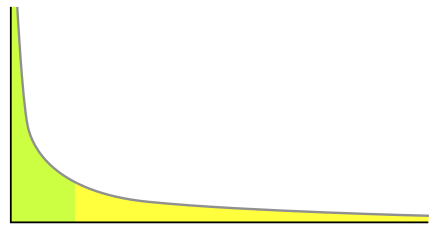
\includegraphics[width=4cm, height=3cm]{figures/long_tail.png} \\ \end{center}
The green region to the left represent the few highly rated products and the yellow region represents the unpopular majority. Examples of the long tail (Movielens and Netflix) were shown in class in lecture slides.

{\it Slide 33-43} Group By and Memory Problem\\
$group_by()$ function groups a data frame by specified criteria of rows. Functions such as $filter()$ can be applied to grouped data. We discussed ways that different data can be grouped. There may be situations when grouped data is too larged to be stored in memory. Streaming algorithms described above can be a potential solution.

\section{Command Line Demo}
\indent Finally, the professor demonstrated command line operations including ls with options, cat, cut, grep, awk, and generating histograms. Demo code can be found on GitHub.





\end{document}

%%% Local Variables:
%%% mode: latex
%%% TeX-master: t
%%% End:
